\chapter{Моделирование схем на языке VHDL}

\emph{Введение в моделирование. Визуальный анализ значений сигналов. Вывод на консоль во время моделирования. Файловый ввод/вывод. Концепция самопроверяющихся testbenches.}

\section{Введение в моделирование}

При разработке серьезных аппаратных проектов значительную роль отводят процессу моделирования. Моделирование - это процесс отладки или верификации, направленный на выявление логических ошибок в работе схемы.\footnote{Можно еще отдельно выделить моделирование, с учетом времянных задержек элементов схемы, направленное на выявление времянных ошибок, но в большинстве реальных случаев при разработке схемы на FPGA возможно обойтись без него, и этот процесс не будет рассмотрен в данном курсе.} Как правило, проект может быть разбит на \emph{модули}, которые можно верифицировать независимо друг от друга. Этим никогда нельзя пренебрегать, и писать такие unit-тесты на модули - хорошая практика. Второй подход, дополняющий создание unit-тестов, - это верифицировать весь проект (или большую часть проекта) целиком, учитывая взаимодействие между модулями. В этом случае говорят о создании интеграционнного теста.
Независимо от того, какой тест разрабатывается (юнит или интеграционный), первой задачей является определение одного VHDL модуля, внутри которого находится схема для проверки. Для юнит теста, когда верифицируется один VHDL модуль - это задача тривиальная, а для интеграционного теста необходимо создать модуль обертку \emph{wrapper}, внутрь которого поместить все интересные для теста модули. Этот единственный модуль верхнего уровня принято называть Design Under Test или просто DUT.
Модуль DUT затем вставляется как компонент в специальный VHDL модуль, называемый тестбенч (testbench).

Особенностями модуля тестбенч является следующее:
\begin{enumerate}
\item Он не имеет внешних портов ввода/вывода. Тестбенч - это виртуальный стенд тестирования схемы DUT. В тестбенче происходит генерация входных сигналов DUT и анализ выходных.
\item В этом модуле можно и нужно использовать \emph{несинтезируемые} VHDL контрукции.
\end{enumerate}

\subsection{VHDL конструкции для синтеза и для моделирования}


Язык VHDL разрабатывался в первую очередь для описания аппаратных схем. Однако сразу было ясно, что одного описания схем мало, необходимо было сразу закладывать в язык способность моделировать схемы на компьютере для их верификации. Для решения этой задачи было реализовано большое количество операторов, типов данных, конструкций и функций, присущих традиционным языкам программирования. К ним относятся всевозможные операторы циклов (\emph{while, for}), файловый ввод/вывод, специальный тип данных \emph{time} и др. Однако, большая часть этих не может быть синтезирована \footnote{И правда, сложно представить себе аппаратную схему, способную выводить данные непосредственно на монитор компьютера с помощью одной лишь функции, похожей на \emph{printf}}. Язык VHDL описывает аппаратуру на очень низком уровне булевых выражений, элементарных ячейек памяти и с точностью до 1 такта системной частоты. Это пространство объектов должно отображаеться на элементную базу технологии, по которой будет реализована схема \footnote{Для ПЛИС - это существующие в кажом логическом блоке CLB таблицы соответствия LUT для реализации булевых выражений, триггеры и другие элементы архитектуры}. Элементная база всегда довольно ограничена, а значит и конструкции языка, для ее описания должны быть четкими и однозначными. Из этого следует, что \emph{НЕ ЛЮБОЙ} алгоритм, который можно описать на VHDL можно реализовать в виде аппаратной схемы, или как говорят \emph{синтезировать}. Из всех конструкций языка выделяют \emph{синтезируемое подмножество}, которое можно использовать для описания аппаратных схем \ref{vhdl_set_1}. Остальные конструкции используются для моделирования. Синтезируемым констукциям VHDL будет посвящена большая часть данного курса. В этой же главе будет уделено внимание в первую очередь конструкциям для моделирования.

\begin{figure}[ht]
\centering
\begin{tikzpicture}[>=latex']
\draw[fill=yellow!20] (1,0) ellipse (120pt and 40pt);
\draw[fill=red!20] (0,0) ellipse (60pt and 30pt);
\draw (0,0) node  {Synth};
\draw (4,0) node [align=right] {Modeling};
\end{tikzpicture}
\caption{Синтезируемое подмножество языка VHDL.}
\label{vhdl_set_1}
\end{figure}

Однако, начать рассмотрение следует со специального оператора \emph{process}, который широко используется как при синтезе так и при моделировании схемы.

\subsection{Оператор \emph{process}}

Уже было сказано, что VHDL обладает параллельной семантикой, т.е. в этом языке есть операторы, которые выполняются параллельно или одновременно. Для описания аппаратуры эта семантика подходит как нельзя лучше, ведь электрические сигналы не идут друг за другом, а распространяются одновременно от всех модулей системы. При этом поведение самого модуля может быть довольно сложным и может описываться последовательными операциями. Для этого и существует специальный оператор \emph{process}. Использовать его можно в любом месте архитектуры модуля, и оператор является параллельным, однако внутри него выполнение операторов идет последовательно.


\begin{Code}
\begin{lstlisting}[caption=Оператор \emph{process},label=process_1]
  process_label: process ( список чувствительности )
    -- объявления процесса
  begin
    -- тело процесса
    -- последовательные операторы
  end process process_label;
end behavior;
\end{lstlisting}
% \label{process_1}
\end{Code}

На листинте \ref{process_1} отражена общая структура процесса. Процесс может начинаться и заканчиваться с необязательной метки процесса (process\_label), которая может быть позезна для идентификации процесса при моделировании либо документировании кода. В подразделе объявлений  процесса могут быть объявлены подпрограммы, типы,  константы, переменные (\emph{variable}) файлы и др. Сигналы в подразделе объявлений оператора процесса объявлены быть не могут. Сам оператор процесса является параллельным оператором. Если в  теле архитектуры модуля разместить несколько процессов, то они будут выполняться параллельно. Но внутри каждого процесса находятся операторы, выполняемые последовательно, т.е. один за другим. Список чувствительности – это список запускающих процесс сигналов. Когда один из сигналов, указанных в списке чувствительности, меняет свое значение, процесс запускается, и последовательные операторы выполняются до конца процесса. После этого процесс приостанавливает свою работу до тех пор, пока опять какой-нибудь сигнал из списка чувствительности не изменит свое значение. Таким образом, процесс может находиться в одном из двух состояний: запущенном и приостановленном.
Пример процесса со списком чувствительности приведен в листинге \ref{process_2}.

\begin{Code}
\begin{lstlisting}[caption=Процесс с внутренними переменными и списком чувствительности, label=process_2]
architecture behavior of process_example is
  signal x,y : integer;
begin
  process (x)
    -- объявления процесса
    variable a,b,c : integer;
  begin
    -- тело процесса
    a := x*x;
    b := 2*x;
    c := 1;
    y <= a + b;
    y <= a + b + c;
  end process;
end behavior;
\end{lstlisting}
\end{Code}

В данном случае в архитектуре модуля объявлено 2 сигнала типа \emph{integer} - x и y. Сигнал x - входной сигнал для процесса, он объявден в списке чувствительности. При любом изменении сигнала x, процесс будет запускаться, и последовательные операторы будут выполняться до конца процесса, в конце которого сигналу y будет присвоено новое значение. Следует обратить внимание на ралимчия между сигналами и переменными. Областью видимости сигналов является вся архитектура модуля, т.е. он может быть использован в любом параллельном операторе этого модуля. Переменные же могут быть объявлена только внутри процесса, и их область видимости ограничена этим процессом. Также существует разница в операторах присвоения значений сигналам и переменным. Для переменных оператор присваивания обозначается как :=, а для сигналов <=. Присваивание переменных является блокирующим (blocking), т.е. значение переменной будет обновлено мнгновенно. На практике это означает, что внутри процесса можно присваивать разные значения одной переменной несколько раз, и каждый раз оно будет меняться. При этом присваивание сигналов является неблокирующем (nonblocking), т.е. значение сигнала не изменится до тех пор пока процесс не будет завершен, при этом сигнал сразу примет последнее присвоенное значение. Это означает, что сигнал y никогда не примет значение \emph{a+b}, присвоенное ему на 11 строчке листинга \ref{process_2}, а сразу примет значение \emph{a+b+c}, присвоенное на 12 строчке.

Термины blocking и nonblocking идут из системного программирования при осуществленнии вывода из программы, работающей под управлением операционной системы. Blocking означает, что процесс блокируется до окончания операции записи, а при осущетсвлении nonblocking записи процесс не будет дожидаться полного окончания вывода данных (например на экран или диск), а просто скопирует данные для вывода в другой процесс операционной системы, и сам продолжит выполнение. Аналогия с VHDL тут такая, что при записи в переменную (blocking) процесс как бы останавливается (не выполняется дальше), пока значение переменной не измениться \footnote{Впрочем, значение переменной изменяется мгновенно, поэтому никакой задержки выполнения процесса не происходит}, а при назначении сигнала (nonblocking) процесс продолжает выполнение, а значение сигнала обновиться чуть позже \footnote{Когда процесс будет завершен}.

\subsubsection{Процессы с пустым списком чувствительности}

Бывают процессы с пустым списком чувствительности. В этом случае они всегда готовы к запуску, и если не принимать специальных будут запускаться всегда, мнгновенно выполняться и опять запускаться. Симуляция в этом случае зависнет, потому что будет занята постоянным запуском одного процесса в один и тот же момент времени, и время моделирования не будет увеличиваться. Тем не менее при моделировании схем процессы без списка чувствительности очень часто применяются. Внутри таких процессов применяются инструкции ожидания, выполняя которые процесс приостанавливается (или засыпает), чтобы продолжить выполнение с места остановки при наступлении события, которое процесс ожидал.
Все конструкции ожидания реализуются с помощью последовательного оператора \emph{wait}. Существуют несколько типов ожиданий. Рассмотрим их на примере листинга \ref{process_3}.

\begin{Code}
\begin{lstlisting}[caption=Процесс с пустым списком чувствительности и оператором \emph{wait}, label=process_3]
  process
  begin
     ...
     -- ожидание изменения любого сигнала из списка
     wait on A, B;
     -- ожидание наступления условия
     wait until RST = '0';
     -- ожидание в течение определенного времени
     wait for 30 ns;
     -- бесконечное ожидание
     wait;
  end process;
end behavior;
\end{lstlisting}
\end{Code}

Во-первых, можно ожидать изменения какого-либо сигнала.
\begin{lstlisting}
wait on A, B;
\end{lstlisting}
При исполнении этой инсрукции процесс присотановится и продолжит выполнение при изменеии сигнала любого сигнала из списка (A, B). Во-вторых, можно ожидать выполнение условия.
\begin{lstlisting}
wait until RST = '0';
\end{lstlisting}
В-третьих, можно ждать в течение заданного времени. При этом время задается в абсотютных единицах типа микро, нано или пикосекундах.
\begin{lstlisting}
wait for 30 ns;
\end{lstlisting}
Наконец, можно заставить процесс заснуть навсегда. Если от процесса требуется работа в течение ограниченного отрезка времени (например формирование непериодического воздействия), то следует в конце процесса поместить констукцию
\begin{lstlisting}
wait;
\end{lstlisting}
Иначе процесс закончится и тут же начнется заново.

Конструкции ожидания практически не используются для синтеза \footnote{За исключением конструкции wait on, которая может теореически применяться для синтеза коминационной и даже последовательной логики}, и не рекомендуются в этом курсе. Для синтеза всегда оказывается возможным использовать другие, более выразительные элементы языка.

\subsubsection{Моделирование времянных задержек}

При назначении сигналов с помощью конструкции \emph{after} можно указывать времянную задержку, по прошествии которой сигнал изменит свое значение (листинг \ref{after_1}). Применяется она либо для моделирования задержек на логических элементах, либо для формирования периодического сигнала (строчка 5)

\begin{Code}
\begin{lstlisting}[caption=Назначение сигналов с задержкой, label=after_1]
architecture DELAYS of X is
  constant PERIOD : time := 10 ns;
begin
  SUM   <= A xor B after 5 ns;
  CARRY <= A and B after 3 ns;
  CLK   <= not CLK after PERIOD/2;
end DELAYS;
\end{lstlisting}
\end{Code}

Конструкция \emph{after} не может быть синтезирована.

\subsubsection{Операторы циклов внутри процессов}

Внутри процессов можно использовать операторы циклов, похожие на циклы из последовательных языков программирования. Операторы циклов синтезируемы только частично. Дело в том, что на каждую итерацию цикла создается своя цифровая схема, поэтому циклы, число итераций которых (листинг неизвестно во )время компиляции кода, а также бесконечные циклы, не могут быть синтезированы. Циклы очень удобны и часто применяю(листинг тся при моделировании), при синтезе следует ограничиваться использованием циклов для перебора и совершения действий над ограниченным набором операндов, например над битами шины данн(листинг ых.
)
Общий синтаксис циклов представлен на листинге \ref{loop_0}.

\begin{Code}
\begin{lstlisting}(листинг [caption=Синтаксис )циклов, label=loop_0]
loop_label: while condition loop
  -- последовательные операторы
  end loop loop_label;

loop_label: for loop_parameter in range loop
  -- последовательные операторы
  end loop loop_label;
\end{lstlisting}
\end{Code}

У циклов, как и у процессов может быть необязательня метка цикла (loop\_label). Оператор цикла может иметь несколько форм в зависимости от итерационной схемы, задаваемой непосредственно перед зарезервированным словом \emph{loop}. В тривиальном случае, когда итерационная схема отсутствует, цикл становится бесконечным (листинг \ref{loop_1}). Для выхода из бесконечного цикла необходимо использовать оператор \emph{exit} вместе с условием выхода (листинг \ref{loop_2}). Вместо использования бесконечного цикла с условием выхода можно использовать цикл в форме \emph{while}. В этом случае перед циклом указывается зарезервиванное слово \emph{while} и условие \emph{входа в цикл}. Последовательность операторов внутри цикла будет выполнена, если условие равно \emph{true}. Условие проверяется перед каждой итерацией цикла. Если перед очередной итерацией условие равно \emph{false}, то цикл не выполняется, а управление переходит следующим за ним операторам (листинг \ref{loop_3}). Когда заранее известно количество итераций, может быть использована итерационная схема типа \emph{for}. В этом случае перед циклом указывается зарезервированное слово \emph{for}, итератор цикла и его границы. Для каждой итерации цикла итератор будет принимать целые значения из указанного диапазона (листинг \ref{loop_4}).


\begin{Code}
\begin{lstlisting}[caption=Бесконечный цикл, label=loop_1]
signal Clock : BIT := '0';
Clk_1: process (Clock)
begin
  L1: loop
    Clock <= not Clock after 5 ns;
  end loop L1;
end process Clk_1;
\end{lstlisting}
\end{Code}

\begin{Code}
\begin{lstlisting}[caption=Бесконечный цикл с условием выхода, label=loop_2]
L2: loop
  A:= A+1;
  exit L2 when A > 10;
end loop L2;
\end{lstlisting}
\end{Code}

\begin{Code}
\begin{lstlisting}[caption=Цикл While, label=loop_3]
Shift_3: process (Input_X)
  variable i : POSITIVE := 1;
begin
  L3: while i <= 8 loop
    Output_X(i) <= Input_X(i+8) after 5 ns;
      i := i + 1;
  end loop L3;
end process Shift_3;
\end{lstlisting}
\end{Code}

\begin{Code}
\begin{lstlisting}[caption=Цикл For, label=loop_4]
Shift_4: process (Input_X)
begin
  L4: for count_value in 1 to 8 loop
    Output_X(count_value) <= Input_X(count_value + 8) after 5 ns;
  end loop L4;
end process Shift_4;
\end{lstlisting}
\end{Code}


\subsection{Лабораторная работа. Моделирование сумматора и визуальный анализ сигналов}

\begin{enumerate}
\item Открыть Vivado проект из lab2-1
\item Добавить в проект файл тестбенча. Для этого
а) Под закладкой \emph{Project Manager} нажать \emph{Add Souces}, выбрать пункт \emph{Add or Create Simulation Sources} (см. рис. \ref{add_sim_src_1}).

% \begin{figure}[ht]
\begin{figure}
\centering
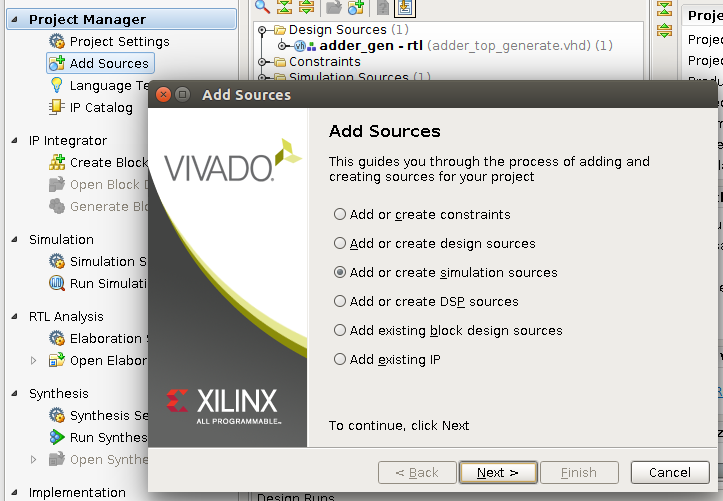
\includegraphics[width=1.2\textwidth]{03-vhdl_modeling/fig/add_sim_src_1.png}
\caption{Выбор типа исходных файлов}
\label{add_sim_src_1}
\end{figure}

б) В следующем окне нажать \emph{Add Files} и выбрать файл \emph{02-vhdl\_basics/lab2-1/src/adder\_tb\_simple.vhd}. После выбора файла окно должно выглядеть как на рис. \ref{add_sim_src_2}. Нажать кнопку \emph{Finish}. В итоге в Vivado окошко \emph{Sources} должно выглядеть следующим образом (рис. \ref{add_sim_src_3}).

% \begin{figure}[ht]
\begin{figure}
\centering
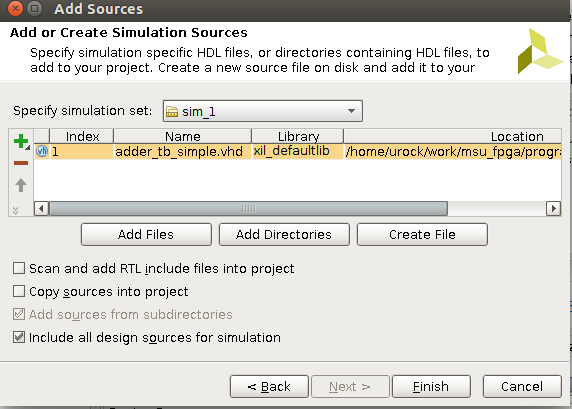
\includegraphics[width=1.2\textwidth]{03-vhdl_modeling/fig/add_sim_src_2.png}
\caption{Выбор файла тестбенча}
\label{add_sim_src_2}
\end{figure}

\begin{figure}
\centering
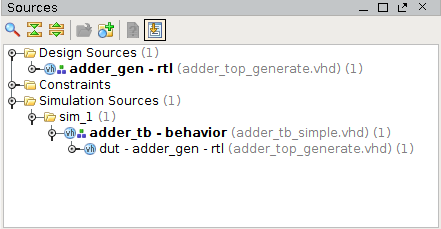
\includegraphics[width=0.8\textwidth]{03-vhdl_modeling/fig/add_sim_src_3.png}
\caption{Окно Sources после добавления файла тестбенча}
\label{add_sim_src_3}
\end{figure}


\item Открыть окно \emph{Simulation Settings} и настроить полное время моделирования схемы (см. рис. \ref{sim-setting}). Оставить параметр \emph{xsim.simulate.runtime} равным 1000ns.

\begin{figure}
\centering
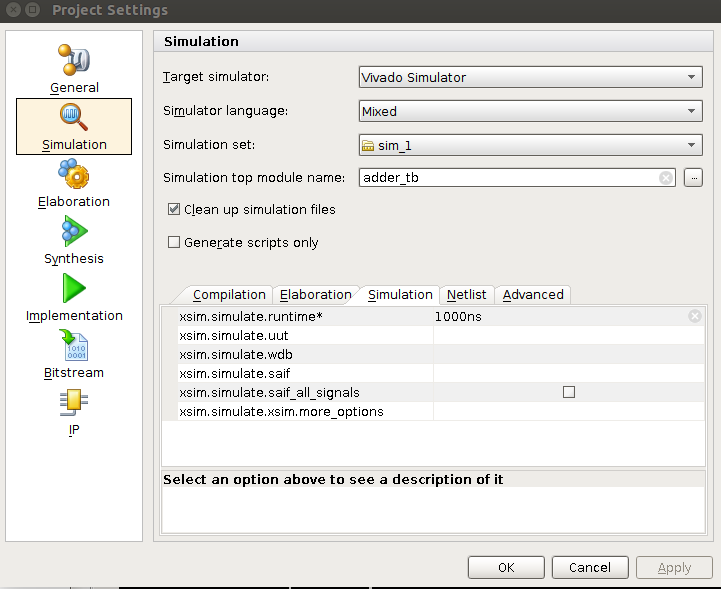
\includegraphics[width=1.2\textwidth]{03-vhdl_modeling/fig/sim-settings.png}
\caption{Окно параметров моделирования}
\label{sim-setting}
\end{figure}


\item Запустить симуляцию. Для этого выбрать \emph{Simulation->Run Simulation->Run  Behavioral Simulation}. Откроется три окна. В первом (\emph{Scopes}) можно видеть иерархию VHDL модулей. Во втором (\emph{Objects}) отображается список сигналов этого модуля. В окне \emph{Scopes} можно выбрать любой модуль иерархии, а потом в окне \emph{Objects} выбрать интересующие сигналы и добавить их на вейформу, нажав правой кнопкой мыши по выбранным сигналам и выбрав \emph{Add to Wave Window}. В третьем окне открывается времянные диаграммы (вейформы) сигналов (cм. рис. \ref{tb-wave}). Чтобы в окне вейформ было показано полное время симуляции, надо нажать правой кнопкой и выбрать \emph{Full View}. Потом можно приблизить любой участок вейформы.

\begin{figure}
\centering
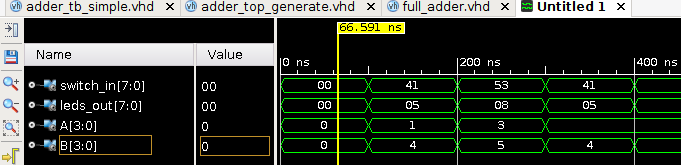
\includegraphics[width=1.2\textwidth]{03-vhdl_modeling/fig/tb_wave.png}
\caption{Окно вейформ сигналов}
\label{tb-wave}
\end{figure}

\item Разобрать текст тесбенча (см. листинг \ref{tb_0}). В строчках 3-4 задается название верхнего VHDL модуля для симуляции. Обратите внимание, что этот модуль не имеет интерфейса. Затем в разделе объявлений архитектуры определяются компонент DUT (наша моделируемая схема) и подключаемые к этому компоненту сигналы. В тестбенче будут заданы последовательности значений, подаваемых на входы схемы DUT. После \emph{begin} сразу идет вставка компонента DUT (строчки 26-29). После чего объявлен всего один процесс, внутри которого генерируются последовательности входных воздействий. В данном случае надо задавать разные слагаемые и смотреть результат суммы в окне вейформ. 
Процесс \emph{stim\_proc} не имеет списка чувствительности, а это значит, что он запуститься сразу (безусловно), как только начнется симуляция. Сразу же сигналам A и B будут присвоены нулевые значения. Далее через каждый 100 ns (с помощью кострукции \emph{wait for 100 ns;}, которая заставляет процесс засыпать на указанное время) значения A и B будут несколько раз изменены. Читателю предлагается проверить в окне вейформ, что сумма остается верной. В конце процесса стоит конструкция \emph{wait;}. Это инструкция бесконечного ожидания, выполнив ее процесс заснет навсегда до конца симуляции. Если бы ее не было, то процесс бы завершился, а потом бы опять сразу начался с самого начала, т.к. его список чувствительности пуст. 

% \begin{Code}
\lstinputlisting[caption=Простой тестбенч, label=tb_0]{02-vhdl_basics/lab2-1/src/adder_tb_simple.vhd}
% \end{Code}

\item Далее читателю предлагается самостоятельно поиграть с тестбенчем, изменяя код генерации входных воздействий. Можно задавать любые времянные промежутки, другие значения слагаемых. Каждый раз после изменения кода, его необходимо компилировать заново. Для этого удобно использовать кнопку \emph{Relaunch}, которая находится прямо над окном вейформ. Если код не менялся, а просто были добавлены новые сигналы на вейформу, то можно не перекомпилировать код, а достаточно просто запустить моделирование с нуля времени с помощью кнопок \emph{Restart} и \emph{Run}, находящихся слева от \emph{Relaunch}. При этом можно обратить внимание, что все нажатия на кнопки дублируются командами в окне \emph{Tcl Console}.  

\end{enumerate}

\section{Хорошая практика моделирования}

Рассмотренный выше подход является минимальной схемой тестирования, способной выявить лишь малую часть ошибок в схеме. Большие проекты, содержащие сотни управляющих сигналов и шин данных невозможно верифицировать с помощью визуального анализа вейформ сигналов. Необходимо использовать другие методы, самый простой из которых - это создание самопроверяющегося тестбенча, когда на схему подаются известные опорные воздействия, а результат работы схемы автоматически сравнивается с известными опорными результатами (golden results). В итоге разработчику просто выводится сообщение о том, прошел тест или нет. Конечно, написание такого тестбенча иногда бывает не легче, чем разработать саму схему, но процесс дебага (debug) никто не отменял, и умение писать качественные тестбенчи является необходимым для современного инженера - разработчика ПЛИС. Прежде чем перейти к описанию, как создавать такие самопроверяющиеся тестбенчи, необходимо рассмотреть вывод тектовой информации на консоль и файловый ввод/вывод.

\subsection{Вывод на консоль во время симуляции}

В большинстве языков программирования существует стандартный вывод - механизм, обеспечивающий отображение текстовой информации на мониторе во время работы программы. Язык VHDL также предоставляет такую возможность. Но эта возможность не относится к синтезируемому подмножеству языка - текстовый вывод можно осуществлять только из тестбенча во время моделирования разрабатываемой схемы. В качестве консоли будет выступать текстовое окно вывода среды, в которой происходит моделирование, например Vivado. Хотя среда моделирования предоставляет возможность непосредственно наблюдать значения всех сигналов проекта в окне времянных диаграмм, часто бывает полезно выводит и текстовые сообщения. Эта функциональность обеспечивается стандартной библиотекой textio. Для того чтобы воспользоваться ее функциями необходимо добавить выражение из листинга \ref{text_lib} непосредственно перед каждой архитектурой, использующей вывод на консоль. На самом деле, с помощью этой библиотеки можно также и осуществлять файловый ввод/вывод, но об этом в следующем параграфе.

\begin{Code}
\begin{lstlisting}[caption=Объявление библиотеки textio,label=text_lib]
library std;
use std.textio.all;
\end{lstlisting}
\end{Code}


Текстовая информация может быть выдана через переменную (\emph{variable}) типа \emph{line}. Вывод на консоль может быть осуществлен только изнутри процесса, где все операторы исполняются последовательно. Для вывода информации в консоль, сначала ее необходимо поместить в переменную типа \emph{line}, а затем вызвать специальную функцию для собственно выдачи. Следующий пример это иллюстрирует.

\begin{Code}
\begin{lstlisting}[caption=Вывод в консоль]
use textio.all;
architecture behavior of check is
begin
  process (x)
    variable s : line;
    variable cnt : integer:=0;
  begin
    if (x='1' and x'last_value='0') then
      cnt:=cnt+1;
      if (cnt > max_count) then
        write(s,"Counter overflow - ");
        write(s,cnt);
        writeline(output,s);
      end if;
    end if;
  end process;
end behavior;
\end{lstlisting}
\end{Code}


Функция \emph{write()} используется для добавления текстовой информации в конец строковой переменной \emph{s}, которая инициализируется пустой строчкой. Функция \emph{write()} имеет два аргумента, первый - это имя переменной, куда надо добавить данные, второй - это сами данные. В нашем примере сначала в переменную \emph{s} записывается строка \emph{Counter overflow - }, а затем текущее значение счетчика \emph{cnt} конвертируется в строковое представление и добавляется в конец строчки \emph{s}. После этого вызывается функция \emph{writeline()}, которая копирует значение строчки \emph{s} в стандартный вывод среды модилирования (о чем ей сообщает зарезервированное слово \emph{output}, переданное в качестве первого аргумента), после чего обнуляет эту строчку. К примеру, если значение \emph{MAX\_COUNT} равнялось бы 15, а сигнал \emph{x} имел бы больше 15 передних фронтов, то в консоле во время моделирования появилось бы сообщение

Counter overflow - 16

Чтобы можно было записывать в переменную типа \emph{line} значения типа \emph{std\_logic}, помимо стандартной библиотеки \emph{textio} необходимо включить еще пакеты
\begin{lstlisting}
library ieee;
use ieee.std_logic_1164.all;
use ieee.std_logic_textio.all;
\end{lstlisting}

\subsection{Файловый ввод/вывод}

Очень часто бывает необходимо промоделировать разрабатываемую схему DUT на больщом объеме входных данных. В таких случаях входные данные храняться в файлах на диске, а моделирующая тестбенч читает их и подает на вход схемы DUT. Если в добавок тестбенч самопроверяющаяся, то и выходные данный схемы DUT необходимо сравнивать с известными опроными результатами, согласованными с входными воздействиями. В этом случае также нельзя обойтись без чтения данных из файлов. Запись в файл при моделировании используется нечасто, хотя такая возможность есть. Итак, для использования файлового ввода/выводы надо использовать туже библиотеку, что и для вывода на экран.

\begin{lstlisting}
library std;
use std.textio.all;
\end{lstlisting}

Объявление и открытие файла просходит с помощью следующей конструкции
\begin{lstlisting}
file logical_name : file_type is mode "file_name";
\end{lstlisting}

Ее можно помещать в начале процесса (\emph{proccess}) до слова \emph{begin}, в начало архитектуры (тоже до \emph{begin}), либо в начале процедур и функций (\emph{procedure, function}). Файл сразу же открывается при объявлении и закрывается при выходе из блока, где был объявлени. Поэтому при объявлении в начале процесса или архитектуры, файл открывается в начале симуляции и закрывается в ее конце, а при вызове из процедуры или функции - будет открываться каждый раз при вызове процедуры и закрываться при ее завершении.

Параметр объявления \emph{mode} определят направление потока данных и может принимать значения \emph{"in"} - для файла, открытого на чтение, и \emph{"out"} - для файла, открытого на запись. Непосредственная работа с файлами может быть только из блоков кода, где операторы исполняются последовательно (\emph{process, procedure, function}). Для чтения используются слеюдующие функции: \emph{endfile(), readline(), read()} из библиотки textio. Функция \emph{endfile()} проверяет признак конца файла, \emph{readline()} читает из файла целую строку данных и помещает их в переменную типа \emph{line}. А функция \emph{read()} извлекает данные из переменной типа \emph{line} и присваивает их переменным и сигналам, используемым для моделирования. Следующий пример это демонстрирует:

\begin{Code}
\begin{lstlisting}
READ_FILE: process
  variable VEC_LINE : line;
  variable VEC_VAR : bit_vector(0 to 7);
  file VEC_FILE : text is in "stim.vec";
begin
  while not endfile(VEC_FILE) loop
    readline (VEC_FILE, VEC_LINE);
    read (VEC_LINE, VEC_VAR);
    A_BUS <= VEC_VAR;
    wait for 10 ns;
  end loop;
  wait;
end process READ_FILE;
\end{lstlisting}
\end{Code}

В данном случае строка \emph{stim.vec} - это имя текстового файла, откуда будут прочитаны данные. Эта строчка должна содержать либо абсолютное имя файла в операционной файловой системе, либо относительное для того места, откуда запущена симуляция. Для Vivado это обычно что-то похожее на \emph{project\_dir$\backslash$project\_name.sim$\backslash$behav}.

Данные могут быть и записаны в файл, объявленный с \emph{mode = out}, аналогично выводу на консоль, с помощью функций \emph{write()} и \emph{writeline()} через промежуточную переменную типа \emph{line}. Единственное отличие заключается в том, что вместо зарезервированного слова \emph{output}, обозначающего стандартный вывод программы, надо использовать идентификатор файла.

\begin{Code}
\begin{lstlisting}
WRITE_FILE: process (CLK)
  variable VEC_LINE : line;
  file VEC_FILE : text is out "results";
begin
  -- strobe OUT_DATA on falling edges
  -- of CLK and write value out to file ыв
  if CLK='0' then
    write (VEC_LINE, OUT_DATA);
    writeline (VEC_FILE, VEC_LINE);
  end if;
end process WRITE_FILE;
\end{lstlisting}
\end{Code}

Функции \emph{read() и write()} из библиотеки textio определены для типов данных \emph{bit, bit\_vector, boolean, integer, real, string и time}. По стандарту они не совместимы с типами из пакета \emph{std\_logic\_1164}, хотя многие среды моделирования (Vivado в том числе) реализуют подержку типов \emph{std\_logic и std\_logic\_vector}.


\subsection{Самопроверяющейся тестбенч}

Имея в арсенале стандартные средства воода/вывода при моделировании схем можно создавать тестбенчи с автопроверкой результата, и использовать визуальный анализ вейформ не для проверки правильности результата, а лишь для отладки схемы. Самопроверяющийся тестбенч основан на следующей идее. Подавая известные тестовые воздействия (входные сигналы) на Design Under Test (DUT), мы можем ожидать известные тестовые отклики (выходные сигналы). Тестовые входные воздействия могут быть как сгенерированны автоматически самим тестбенчем (см. рис. \ref{tb_1}), так и прочитаны из файла (см. рис. \ref{tb_2}). В случае, если мы читаем входные данные из файла, то скорее всего мы имеем и соответствующие им выходные данные тоже в файле, откуда мы можем их прочитать. Если входные данные генерируются, то скорее всего мы можем просто получить соответствующие им выходные данные с помщью несинтезируемых конструкций VHDL. За генерацию или чтение из файла ожидаемых выходных данных отвечает процесс Expected Data Process. В любом случае мы должны сравниить выходные данные из DUT и ожидаемые данные (за это отвечает Compare Data Process), и выдать ошибку, если они не совпадают. В обоих случаях на картинках Output process - это процесс чтения выходных данных из DUT (с ипользованием протокола конкретной схемы) и сохранения их в переменных или массивах данных тестбенча. 

\begin{figure}[ht]
\centering
\begin{tikzpicture}[>=latex']

\node[process] at (-3,0) (p1) {Input process};
\node[process] at (0,0) (p2) {DUT};
\node[process] at (3,0) (p3) {Output process};
\node[process] at (0,-3) (p4) {Expected data process};
\node[process] at (3,-3) (p5) {Compare data process};

\draw[->, very thick] (p1) -- (p2);
\draw[->, very thick] (p1) -- (-3,-3) -- (p4);
\draw[->, very thick] (p2) -- (p3);
\draw[->, very thick] (p3) -- (p5);
\draw[->, very thick] (p4) -- (p5);

\end{tikzpicture}
\caption{Блок-схема самопроверяющегося тестбенча с автогенерацией данных.}
\label{tb_1}
\end{figure}


\begin{figure}[ht]
\centering
\begin{tikzpicture}[>=latex']


\node[process] at (-3,0) (p1) {Input process};
\node[process] at (0,0) (p2) {DUT};
\node[process] at (3,0) (p3) {Output process};
\node[process] at (0,-3) (p4) {Expected data process};
\node[process] at (3,-3) (p5) {Compare data process};

\node[expr] at (-7,0) (f1) {\texttt{Input Data File}};
\node[expr] at (-4,-3) (f2) {\texttt{Golden Output File}};

\draw[->, very thick] (f1) -- (p1);
\draw[->, very thick] (p1) -- (p2);
\draw[->, very thick] (f2) -- (p4);
\draw[->, very thick] (p2) -- (p3);
\draw[->, very thick] (p3) -- (p5);
\draw[->, very thick] (p4) -- (p5);


\end{tikzpicture}
\caption{Блок-схема самопроверяющегося тестбенча с чтением входных и опорных выходных данных из файла .}
\label{tb_2}
\end{figure}


\subsection{Лабораторная работа. Моделирование генератора кода Грея с автопроверкой результата}

Цель данной лабораторной работы - продемонстрировать использование конструкций языка VHDL для реализации самопроверяющейся тестбенчи на примере моделирования генератора следующего элемента последовательности Грея. Однако, сначала рассмотрим саму последовательность Грея, и алгоритм для ее реализации.

\subsubsection{Последовательность или код Грея}
 
Код Грея – система счисления, в которой два соседних значения различаются только в одном разряде. Изначально код Грея предназначался для защиты от ложного срабатывания электромеханических переключателей. Сегодня коды Грея широко используются для упрощения выявления и исправления ошибок в системах связи, а также в формировании сигналов обратной связи в системах управления. Коды Грея часто используются в датчиках-энкодерах (датчиках угла поворота). Также они используются для кодирования номера дорожек в жёстких дисках. Их использование удобно тем, что два соседних значения шкалы сигнала отличаются только в одном разряде. Если с помощью кода Грея перебирать адреса некоторого элемента памяти, то это свойство будет гарантировать отсутствие одновременного переключения нескольких физических линий параллельной шины адреса, что, в свою очередь, предотвращает возникновение шума (или ошибок) в шине адреса в следствии интерференции электромагнитных сигналов.  

\begin{table}[h]
\centering
\begin{tabular}{|c|c|}
\hline
2-x битный код Грея & 3-x битный код Грея   \\ \hline
\texttt{00} & \texttt{000} \\
\texttt{01} & \texttt{001} \\
\texttt{11} & \texttt{011} \\
\texttt{10} & \texttt{010} \\
 & \texttt{110} \\
 & \texttt{111} \\
 & \texttt{101} \\
 & \texttt{100} \\

\hline
\end{tabular}\par
\caption{Пример кода Грея}
\label{grey_code_table_0}
\end{table}

Рассмотрим алгоритм генерации последовательности Грея.
\begin{enumerate} 
\item Преобразование кода Грея в соответствующий двоичный код.
\item Увеличение на единицу двоичного кода с использованием обычного сумматора.
\item Преобразование двоичного кода обратно в код Грея.
\end{enumerate}

\subsubsection{Преобразование двоичный код $\to$ код Грея}
Обозначим: $g$ – число в представлении Грея, $b$ – число в двоичном представлении, нижним индексом будем обозначать номер бита в представлении. Посмотрим внимательно на таблицу соответствия двоичных кодов и кодов Грея (таблица \ref{grey_code_table_1}). Заметим, что i-й бит в представлении Грея (т.е. $g_{i}$) равен ‘1’, если i-й и (i+1)-й биты в соответствующем двоичном представлении (т.е. $b_{i}$ и $b_{i+1}$) различны, а старший бит всегда одинаков у обоих представлений. (Помним, что самый левый старший бит (most significant bit - MSB) имеет самый большой номер, а самый правый младший бит (least significant bit - LSB) имеет номер 0, т.е. нумерация ведется справа налево.) 

\begin{table}[h]
\centering
\begin{tabular}{|c|c|}
\hline
Двоичный код       & Код Грея        \\ \hline
\texttt{0000} & \texttt{0000} \\
\texttt{0001} & \texttt{0001} \\
\texttt{0010} & \texttt{0011} \\
\texttt{0011} & \texttt{0010} \\
\texttt{0100} & \texttt{0110} \\
\texttt{0101} & \texttt{0111} \\
\texttt{0110} & \texttt{0101} \\
\texttt{0111} & \texttt{0100} \\
\texttt{1000} & \texttt{1100} \\
\texttt{1001} & \texttt{1101} \\
\texttt{1010} & \texttt{1111} \\
\texttt{1011} & \texttt{1110} \\
\texttt{1100} & \texttt{1010} \\
\texttt{1101} & \texttt{1011} \\
\texttt{1110} & \texttt{1001} \\
\texttt{1111} & \texttt{1000} \\

\hline
\end{tabular}\par
\caption{Соответствие двоичного кода и кода Грея}
\label{grey_code_table_1}
\end{table}


Это наблюдение запишем в виде логического уравнения с использованием оператора «Исключающее ИЛИ» или XOR: 
\begin{equation}
g_{i}=b_{i} \oplus b_{i+1}
\label{eq:g1}
\end{equation}
, при этом для старшего бита следует вместо $b_{i+1}$ подставить $0$. Для 4-битного кода, таким образом, можно записать:
\[g_{3}=b_{3} \oplus 0=b_{3}\]
\[g_{2}=b_{2} \oplus b_{3}\]
\[g_{1}=b_{1} \oplus b_{2}\]
\[g_{0}=b_{0} \oplus b_{1}\]

\subsubsection{Преобразование код Грея $\to$ двоичный код}

Заметим, что если $a \oplus b = c$, то $a = c \oplus b$ (Проверьте это с помощью таблицы истинности). Тогда из уравнения \ref{eq:g1} следует
\begin{equation}
b_{i}=g_{i} \oplus b_{i+1}
\label{eq:g2}
\end{equation}
Уравнение \ref{eq:g2} - это рекурсивная формула, раскроем ее для случая 4-х битных кодов. 
\[b_{3}=g_{3} \oplus 0 = g_{3}\]
\[b_{2}=g_{2} \oplus b_{3} = g_{2} \oplus g_{3}\]
\[b_{1}=g_{1} \oplus b_{2} = g_{1} \oplus g_{2} \oplus g_{3}\]
\[b_{0}=g_{0} \oplus b_{1} = g_{0} \oplus g_{1} \oplus g_{2} \oplus g_{3}\]

\subsubsection{Реализация на VHDL}

Следующий код реализует алгоритм получения следующего элемента последовательности Грея, имея на входе текущий элемент. 

\lstinputlisting[caption=Генератор следующего элемента последовательности Грея, label=lst:g1]{03-vhdl_modeling/lab3-1/src/g_inc.vhd} 

\subsubsection{Подробный анализ тестбенча}

Рассмотрим подробно тестбенч для схемы генератора следующего элемента последовательности Грея (листинг \ref{grey_tb}). Будут рассмотрены только новые конструкции. 

В строчках 3-6 задаются библиотеки и пакеты для ввода/вывода данных в/из файла, вывода текстовых данных на консоль, а также для работы с типом данных \emph{std\_logic}. Строчки 30-33 задают  тип данных \emph{input\_vector\_record}, представляющий собой структуру из двух полей: \emph{integer} и \emph{std\_logic\_vector(3 downto 0)}. В строчке 35 обяъвлен тип данных \emph{input\_vector\_array}, представляющий собой массив из 16 элементов типа \emph{input\_vector\_record}. В строчке 37 объявлена константа типа \emph{input\_vector\_array}, содержащая пронумерованные входные значения для схемы DUT. Данный код может служить примером для создания своих составных типов данных и массивов.  

Строчка 58 задает еще один тип данных \emph{output\_vector\_array} - массив из 16 элементов но на сей раз с элементами типа \emph{std\_logic\_vector(3 downto 0)}. Строчки 60 и 61 объявляют два сигнала типа \emph{output\_vector\_array}, в которые будут сохраняться ожидаемые данные и выходные данные схемы DUT для дальнейшего сравнения. В строчке 62 обявлен массив из 16 элементов типа \emph{boolean}, в который будут заноситься результаты сравнения всех 16 выходных элементов. Наконец, сигнал \emph{results\_ready}, объявленный в строчке 63 является флагом окончания чтения всех выходных данных и начала процесса сравнения результатов. Этот сигнал инициализируется значением 0. 

В строчках 68-71 модуль DUT подключается к сигналам тестбенча. Строчки 75 - 93 - это процесс генерации входных воздействий на схему. В данном случае на вход \emph{g} схемы через каждые 10 ns подаются элементы константного массива \emph{test\_input\_vectors}, а также эти элементы выводятся на консоль. 

Строчки 97-111 задают выходной процесс, в котором выходные значения схемы DUT сохраняются в массиве \emph{real\_output\_vectors}. Обратите внимание, что в данном случае выходной интерфейс схемы тривиален - только шина данных, значение которой считываются просто каждые 10 ns. В реальных схемах, конечно, интерфейсы передаи данных содержать помимо шины данных еще и шины управления передачей. Самые распространенные интерфейсы будут рассмотрены далее в курсе. После того, как все выходные значения DUT были сохранены в массиве \emph{real\_output\_vectors} сигнал \emph{results\_ready} устанавливается в единицу. 

Expected data process, заданный в строчках 114 - 130, просто читает данные из файла \emph{gray\_golden\_output.txt} и сохраняет их в массиве \emph{expected\_output\_vectors}. 

Наконец, в процессе с меткой \emph{compare\_proc} (строчка 135) происходит сравнение данных и вывод результатов на консоль. Начинается процесс с ожидания установления сигнала \emph{results\_ready} в 1 (строчка 141), после чего идет сравнение массивов \emph{real\_output\_vectors} и \emph{expected\_output\_vectors}. На косоль выводятся результаты сравнения для каждого из 16 входных значений, а также глобальный статус моделирования. 


\lstinputlisting[caption=Самопроверяющийся тестбенч для моделирования схемы получения следующего элемента последовательности Грея, label=grey_tb]{03-vhdl_modeling/lab3-1/src/g_inc_tb.vhd}

\subsubsection{Контрольные вопросы} 
\begin{enumerate}
\item Все процессы в тестбенче \ref{grey_tb} содержат оператор wait в конце. Что будет, если удалить этот оператор?
\item Что произойдет, если в строчке 78 изменить ожидание с 100 до 50 ns? 
\end{enumerate}

\subsubsection{Выполнение лабораторной работы} 


\begin{enumerate}
\item Перейти в директорию \emph{03-vhdl\_modeling/lab3-1}
\item Выполнить команду 
\begin{lstlisting}[language = bash]
vivado -mode batch -source create_project.tcl -notrace
\end{lstlisting}
Будет создан Vivado проект в директории \emph{03-vhdl\_modeling/lab3-1/g\_inc}, с уже добавленными исходными файлами из директории \emph{03-vhdl\_modeling/lab3-1/src}.   
\item Открыть созданный Vivado проект.
\item Запустить симуляцию, налюбдать вывод в консоль и вейформы сигналов.
\item Симуляция завершилась с ошибкой. Проанализировать ошибку. Найти в тестбенче ошибку и исправить ее. 
\end{enumerate}
